\documentclass[11pt]{report} 
\usepackage{titlesec}
\usepackage{diagbox}
\usepackage{makecell}

%--------------------------- Chapter layout  ----------------------%
\titleformat{\chapter}
  {\normalfont\LARGE\bfseries}{\thechapter}{1em}{}
\titlespacing*{\chapter}{0pt}{3.5ex plus 1ex minus .2ex}{2.3ex plus .2ex}
%----------------------------------------------------------------------%

%\documentclass[paper=a4,fontsize=11pt]{scrartcl}	 			% KOMA-article class
							
%\usepackage[english]{babel}								% English language/hyphenation
%\usepackage[protrusion=true,expansion=true]{microtype}		% Better typography
\usepackage{amsmath,amsfonts,amsthm}					% Math packages
\usepackage[pdftex]{graphicx}								% Enable pdflatex
\usepackage[svgnames]{xcolor}							% Colors by their 'svgnames'
\usepackage{geometry}
	\textheight=700px									% Saving trees ;-) 
\usepackage{url}										% Clickable URL's
\usepackage{wrapfig}									% Wrap text along figures

\usepackage[colorinlistoftodos,prependcaption]{todonotes}


\frenchspacing									% Better looking spacings after periods
%\pagestyle{empty}								% No pagenumbers/headers/footers
%\usepackage{bbding}									% Symbols


% ------- Enable UTF8 characters ------- %
%\usepackage[utf8]{inputenc}
\usepackage[english]{babel}

\setlength\parindent{0pt}

\usepackage{listings}
\usepackage{color}

%\usepackage{pdfpages}

% ------------ Code Listing ------------- %

\definecolor{dkgreen}{rgb}{0,0.6,0}
\definecolor{gray}{rgb}{0.5,0.5,0.5}
\definecolor{mauve}{rgb}{0.58,0,0.82}

\lstset{frame=false,
  language=C++,
  aboveskip=3mm,
  belowskip=3mm,
  showstringspaces=false,
  columns=flexible,
  basicstyle={\small\ttfamily},
  numbers=none,
  numberstyle=\tiny\color{gray},
  keywordstyle=\color{blue},
  commentstyle=\color{dkgreen},
  stringstyle=\color{mauve},
  breaklines=true,
  breakatwhitespace=true,
  tabsize=3,
  moredelim=**[is][\color{mauve}]{@}{@},
}

% ------- Page layout ------- %
\usepackage{fullpage}
\usepackage{hyperref} % clickable references
\hypersetup{
    colorlinks,
    citecolor=black,
    filecolor=black,
    linkcolor=black,
    urlcolor=black
}
\usepackage{multicol}
\setlength{\columnsep}{1cm}

\usepackage{enumitem}
\usepackage{multirow}

\usepackage{multicol}
\setlength{\columnsep}{0.3cm}

\usepackage{colortbl}

% ------- Images ------- %
\usepackage{graphicx}
\usepackage{caption}
\usepackage{float}
\usepackage{subcaption}
\DeclareCaptionFont{gray}{\color{gray}}
\captionsetup{textfont={footnotesize,sc,gray},font={footnotesize,sc,gray}}
\usepackage{blindtext}
\usepackage[toc,page]{appendix}

% Test

\usepackage{tikz}
\usetikzlibrary{shapes,arrows,shadows}
\newcommand{\mx}[1]{\mathbf{\bm{#1}}} % Matrix command
\newcommand{\vc}[1]{\mathbf{\bm{#1}}} % Vector command

\usetikzlibrary{arrows}


\title{Stastiscal Machine Learning }


\begin{document}

\begin{titlepage}
\begin{center}


\textsc{\LARGE University of Southern Denmark}\\[1.5cm]
\textsc{\Large Statistical machine learning}\\[0.5cm]
\vfill
\hrule ~\\[0.3cm]
{ \huge \bfseries Exercise 1: kNN\\[0.4cm] }
\hrule ~\\[1.5cm]
\vfill

% Author and supervisor
\noindent
\begin{minipage}{0.4\textwidth}
\begin{flushleft} \large
\emph{Authors:}\\
Keerthikan Ratnarajah
\url{kerat12@student.sdu.dk}\\
Mikael Westermann
\url{miwes12@student.sdu.dk}
\end{flushleft}
\end{minipage}%
\begin{minipage}{0.4\textwidth}
\begin{flushright} \large
\emph{Supervisor:}\\
Norbert Kr\"{u}ger 
\end{flushright}
\end{minipage}

\vspace{1.2cm}
Date: \today


\end{center}
\end{titlepage}

\tableofcontents

\newpage





\bibliographystyle{unsrt}%Used BibTeX style is unsrt

%\begin{appendices}
\section{Introduction}
<<<<<<< HEAD
\todo[inline]{Something...}
The purpose of this report is to develop a system capable of recognizing hand writting characters such as digits (0 - 9).  This report will contain different approaches of classifying this, and their performance.  The dataset used for training and testing the performance of this, has be been made by the students of the statical machine learning class  as seen in \ref{fig:data}. The dataset consist of 400 $\times$ 10 individually handwritten numbers,  provided by each  student of the class.  

\begin{figure}[H]
\centering
\includegraphics[width =0.6\textwidth]{../../SML-database/2016/group2/member1/Ciphers100-0.png}
\caption{Example of the  dataset}
\label{fig:data}
\end{figure} 

The process of recognizing the digits can be divided into 3 steps. 
\begin{itemize}
\item Preprocessing - Extracting the data, and discard irrelevant information. 
\item Feature extraction - Extracting relevant features 
\item Classification - Use the extracted to classify the digits. 
\end{itemize}

=======
>>>>>>> 34ff1c3365fe38aae75203e9098a9fe6bb020ed5

\chapter{kNN}
K - nearest - neighbor or kNN,
is a method for classifying objects based on the distance
to features extracted from ones training data.
The idea in kNN is to identiy k observation which is closest to the new
observation trying to be classified.
 The class with most vote determines which class the new observation
will be classified as. 
K is arbitrarily choosen by the user,
 and has an effect of the peformance of the algorithm. 
k-nn has an optimal classification rate when k becomes very large, 
but will computation wise take more time and vice versa. 
\chapter{Results}
\section{Data collection}

Figure \ref{fig:misalignment} visualizes an example of the data collection.
It is observed that the grid by which digits were separated is misaligned with the grid
in which the digits were written. The black grid becomes part of the digit data.
\begin{figure}[H]
\centering
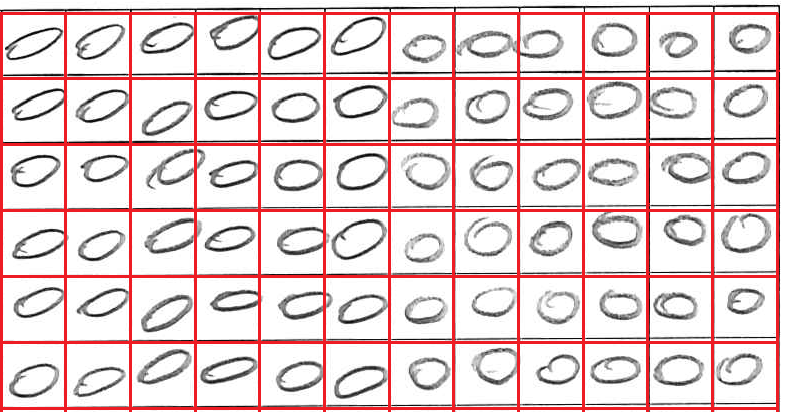
\includegraphics[width  =\textwidth]{figure/kiddi-01-grid-nosmooth-300dpi_cut.png}
\caption{Collected digits. The red grid imposed on the image shows how hand written digits were separated.}
\label{fig:misalignment}
\end{figure}

\section{kNN}
The kNN data processing consists of analyzing the effects of k, smoothing and
DPI density on the error rate  This is found by applying kNN on different training set,
with different smoothing levels, and DPI.

Two smoothing techniques were applied to the images: The average filter, and Gaussian blur.  
For each technique, kNN was applied with different values of k, for which the error rate was calculated.
This allows insight necessary for choosing an optimal k and smoothing parameters.


\begin{table}[h]
% latex table generated in R 3.2.3 by xtable 1.8-2 package
% 
% confusion * 100
% 100 dpi k  = 15
\begin{tabular}{r|rrrrrrrrrr}
%Actual digit
 & 0 & 1 & 2 & 3 & 4 & 5 & 6 & 7 & 8 & 9 \\ 
  \hline
0 & 0.300 & 0.025 & 0.025 & 0.000 & 0.000 & 0.000 & 7.025 & 0.675 & 1.925 & 0.025 \\ 
  1 & 0.000 & 0.675 & 1.325 & 0.000 & 0.000 & 0.000 & 4.475 & 1.950 & 1.400 & 0.175 \\ 
  2 & 0.000 & 0.000 & 2.825 & 0.000 & 0.000 & 0.000 & 1.450 & 3.100 & 2.625 & 0.000 \\ 
  3 & 0.000 & 0.375 & 0.525 & 0.175 & 0.000 & 0.075 & 2.375 & 4.000 & 2.050 & 0.425 \\ 
  4 & 0.025 & 0.050 & 0.025 & 0.025 & 0.175 & 0.025 & 3.700 & 4.250 & 1.475 & 0.250 \\ 
  5 & 0.025 & 0.400 & 0.175 & 0.000 & 0.000 & 1.275 & 4.625 & 0.875 & 2.275 & 0.350 \\ 
  6 & 0.000 & 0.025 & 0.075 & 0.000 & 0.000 & 0.025 & 7.175 & 2.075 & 0.625 & 0.000 \\ 
  7 & 0.000 & 0.125 & 0.725 & 0.000 & 0.000 & 0.075 & 0.275 & 6.675 & 1.775 & 0.350 \\ 
  8 & 0.000 & 0.025 & 0.075 & 0.000 & 0.000 & 0.050 & 5.450 & 1.450 & 2.775 & 0.175 \\ 
  9 & 0.000 & 1.675 & 0.200 & 0.025 & 0.000 & 0.025 & 2.025 & 2.950 & 2.225 & 0.875 \\ 
\end{tabular}
\caption{Confusion matrix. In percent. 100 DPI and average filter smoothing with kernel size 15.}
\label{tb:confusion}
\end{table}
As table
\ref{tb:confusion}

shows, misclassification occurs in several instances.
Notably, digits 6, 7 and 8 are very often misclassified compared to other digits.
The parameters for this test were 100 DPI and average filter smoothing with kernel size 15.

\begin{figure}[H]    
	\begin{minipage}[t]{0.30\textwidth}
		\centering
			
\includegraphics[width=0.4\linewidth]{Figure/mikael_8_2_dpi100_k1.png}
			\caption{DPI = 100 , kernel size = 1}
			\label{fig:dpi_100_1}
	\end{minipage}
	\hspace{\fill}	
	\begin{minipage}[t]{0.30\textwidth}
		\centering
			
\includegraphics[width=0.4\linewidth]{Figure/mikael_8_2_dpi100_k3.png}
			\caption{DPI = 100 , kernel size = 3}
			\label{fig:dpi_100_3}
	\end{minipage}
	\hspace{\fill}
	\begin{minipage}[t]{0.30\textwidth}
		\centering
			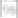
\includegraphics[width=0.4\linewidth]{Figure/mikael_8_2_dpi100_k5.png}
			\caption{DPI = 100 , kernel size =5}
			\label{fig:dpi_100_5}
	\end{minipage}
\vspace*{0.5cm} % (or whatever vertical separation you prefer)	
	\begin{minipage}[t]{0.30\textwidth}
		\centering
			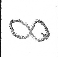
\includegraphics[width=0.4\linewidth]{Figure/mikael_8_2_dpi300_k1.png}
			\caption{DPI = 300 , kernel size = 1}
			\label{fig:dpi_300_5}
	\end{minipage}
\hspace{\fill}	
	\begin{minipage}[t]{0.30\textwidth}
		\centering
			
\includegraphics[width=0.4\linewidth]{Figure/mikael_8_2_dpi300_k5.png}
			\caption{DPI = 300 , kernel size = 5}
			\label{fig:dpi_300_9}
	\end{minipage}	
\hspace{\fill}	
	\begin{minipage}[t]{0.30\textwidth}
		\centering
			
\includegraphics[width=0.4\linewidth]{Figure/mikael_8_2_dpi300_k9.png}
			\caption{DPI = 300 , kernel size = 9}
			\label{fig:dpi_300_9}
	\end{minipage}	
\caption{Effect of smoothing using average filter with different kernel sizes}
\label{fig:average_filter}
\end{figure}

It can be seen based on figure \ref{fig:average_filter} that the smoothing
 filter does have an impact on how clear the digit can be visually
 recognized, and that the higher the DPI density,
  the better visual information. 

Using different smoothing parameters and k, kNN was applied,
using data from one student as training data, and data from another student as testing data.
The correct classification rate was calculated.

\begin{figure}[H]
	\centering
		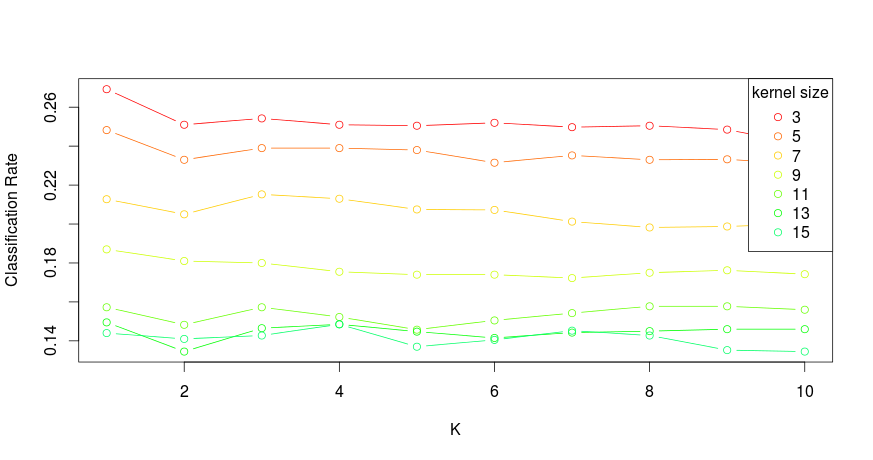
\includegraphics[width = \textwidth]{Figure/data_100_15_10.png}
		\caption{Tested on images with 100 dpi}
		\label{fig:data_100}
\end{figure}

\begin{figure}[H]
	\centering	
		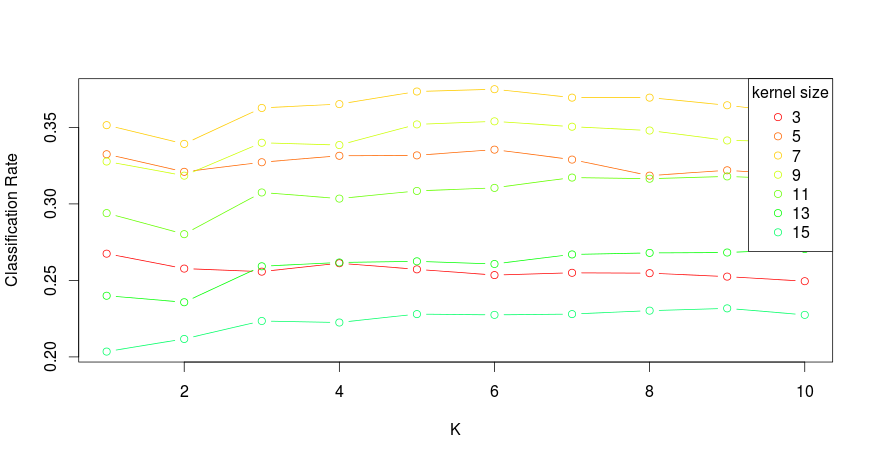
\includegraphics[width = \textwidth]{Figure/data_200_15_10.png}
		\caption{Tested on images with 200 dpi}
		\label{fig:data_200}
\end{figure}

\begin{figure}[H]
	\centering
		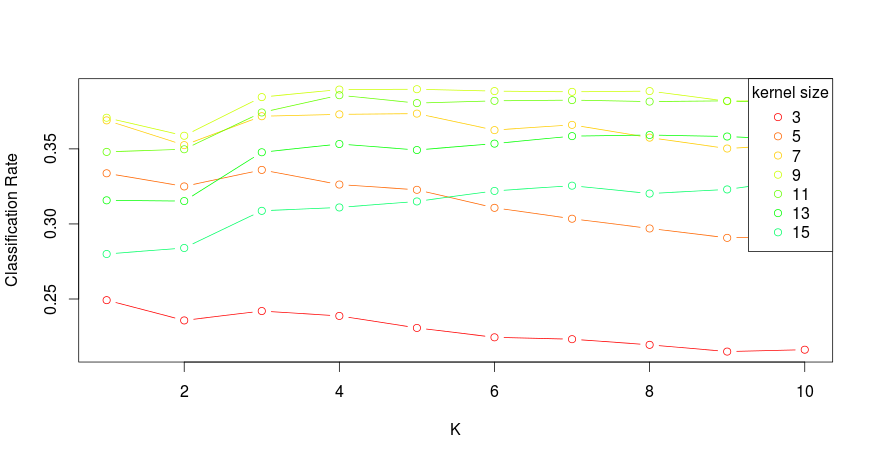
\includegraphics[width = \textwidth]{Figure/data_300_15_10.png}
		\caption{Tested on images with 300 dpi}
		\label{fig:data_300}
\end{figure}

The graphs in figure \ref{fig:data_100} , \ref{fig:data_200}  and \ref{fig:data_300} 
 shows that the images scanned with 300 DPI gives the highest classification rate,
which as previously stated was seen as the ones who gave clearer images as smoothing were applied.
 The graphs shows that the correct classification rate peaks for 100 DPI when applying a kernel at size 3,
 for 200 DPI peaks it is at kernel size 7, and for 300 DPI it peaks at kernel size 9,
 The best perfomance can be found from the images scanned with 300 DPI.
However, very long running times were observed.

\begin{figure}[H]    
	\begin{minipage}[t]{0.30\textwidth}
			\centering
			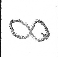
\includegraphics[width=0.4\linewidth]{Figure/mikael_8_2_dpi300_k15_sig_01.png}
			\caption{kernelsize = 15 $\sigma$ = 0.1}
			\label{fig:dpi_300_k_9_s_0.1}
	\end{minipage}
	\hspace{\fill}	
	\begin{minipage}[t]{0.30\textwidth}
		\centering
			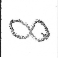
\includegraphics[width=0.4\linewidth]{Figure/mikael_8_2_dpi300_k15_sig_04.png}
			\caption{kernelsize = 15 $\sigma$ = 0.4}
			\label{fig:dpi_300_k_9_s_0.4}
	\end{minipage}
	\hspace{\fill}
	\begin{minipage}[t]{0.30\textwidth}
		\centering
			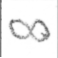
\includegraphics[width=0.4\linewidth]{Figure/mikael_8_2_dpi300_k15_sig_07.png}
			\caption{kernelsize = 15 $\sigma$ = 0.7}
			\label{fig:fig:dpi_300_k_9_s_0.7}
	\end{minipage}
\caption{Effect of smoothing using gaussian filter with different \(\sigma\) values.}
\label{fig:gaussian_filter}
\end{figure}

As an alternative to the average filter could an gaussian filter be used as shown
 in figure \ref{fig:gaussian_filter}. 
Compared to figure \ref{fig:average_filter}, this filter introduces less noise,
and distributes pixel grayscale values more naturally.


\section{Discussion}
\section{Conclusions}
\label{sec:conclusion}
%The main purpose of this project is to compare two classification algorithms,
%k-Nearest Neighbours (k-NN) and Support Vector Machines (SVM),
%for handwritten digit recognition.
%The second purpose of this project is to achieve good classification performance,
%and thus, some preprocessing is needed.
%Lastly, as the digits used in this project
%were written by a class of 23 always competitive students,
%it was chosen to estimate the quality of the hand written digits
%and identify the student with the worst hand writing.
%This required a definition of hand written digit quality,
%which is also presented here.
k-NN with number of neighbours k=5 achieves significantly higher overall 
classification accuracy than SVM with polynomial kernel of degree 2
with scale factor 0.1 and cost of constraints violation C=0.5,
with \(\alpha=0.05\),
when each algorithm is trained with a dataset of hand written digits
from a class of 23 people, and tested on a dataset
with digits written by the same people.
When the training set only contains data from 22 people,
and the test set is written by a person not in the training
set, k-NN does not perform significantly worse
than SVM, although a lower overall accuracy was observed.
Neither does the k-NN classifier perform significantly worse than SVM
when applied to one persons data at a time,
although a lower overall accuracy was observed.

The highest obtained overall classification accuracy is 0.854 with a standard
deviation of 0.0205, for the SVM classifier.

A successful preprocessing scheme involving the perspective transform,
gaussian blur and Principal Component Analysis was implemented.

Person \(G2M1\) (one of the authors) has the worst digit hand writing of the 2016 SML class,
when the writing quality is measured by classification
error on own data. This means \(G2M1\) has the least
within-digit consistent and between-digit varied
hand writing.

%\end{appendices}


\end{document}






















































